\chapter{A Térkép}
Sajnos, mint ahogy az a játék beli terképek többségéről elmondható nem teljesen pontos a Hürtgen-erdő esetében sem. Ezért tapasztalt játékosok előnyt élveznek másokkal szemben, hiszen ők kiismerik magukat a terület környezeti viszonyai között.

Ahogy az a \ref{fig:hurtgenMap}. ábrán látható a terület 15 \emph{Strong Point} található, melyek közül \emph{Háború (Warfare)} játékmódban 5 kerül kiválasztása véletlenszerűen a játék elején - minden két szélességi sávból egy.

\emph{Offenzíva (Offensive)} játékmódban ennél lényegesebben több pontot kell elfoglalniuk a támadóknak.
\begin{figure}
    \centering
    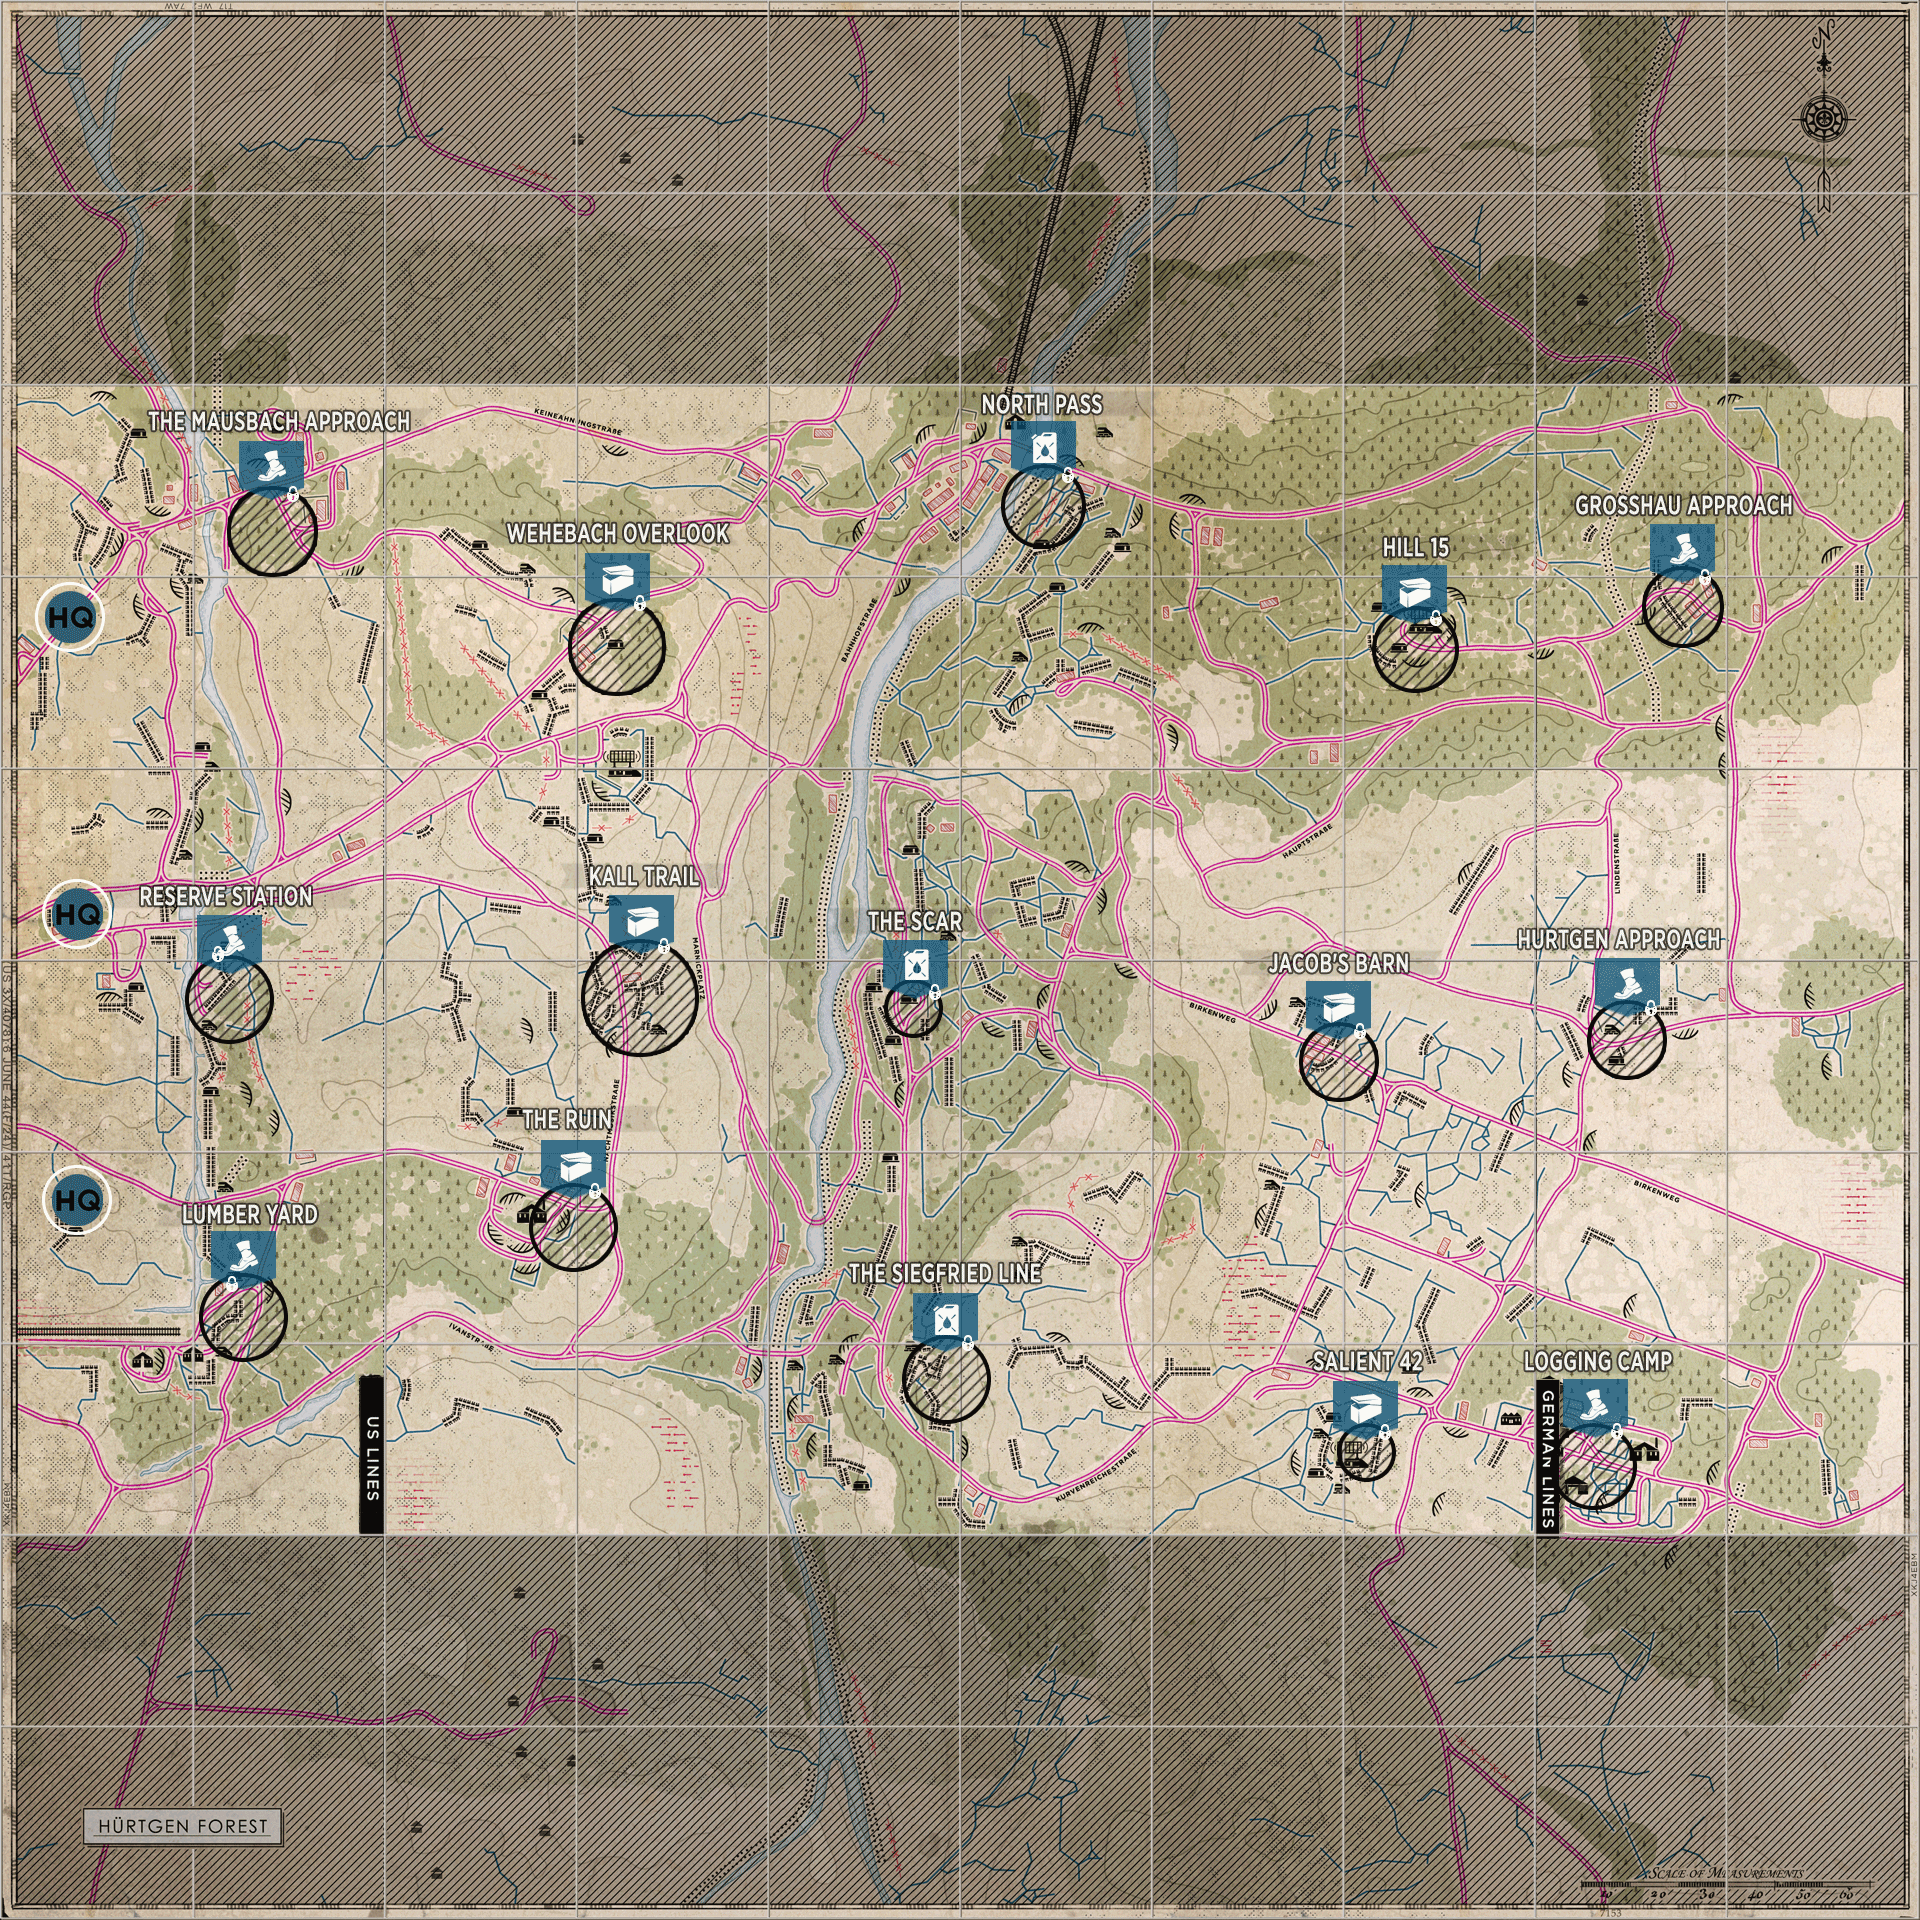
\includegraphics[width=150mm, keepaspectratio]{figures/HurtgenForest.png}
    \caption{Hürtgen-erdő térképe~\cite{WikiHurtgen}}
    \label{fig:hurtgenMap}
\end{figure}

%-----------------------------
\section{Amerikai bázis sáv}
%-----------------------------
\subsection{The Mausbach Approach}

\subsection{Reserve Station}

\subsection{Lumber Yard}

%-----------------------------
\section{Amerikai védekező sáv}
%-----------------------------
\subsection{Wehebach Overlook}

\subsection{Kall Trail}

\subsection{The Ruin}

%-----------------------------
\section{Semleges sáv}
%-----------------------------
\subsection{North Pass}

\subsection{The Scar}

\subsection{The Siegfried Line}

%-----------------------------
\section{Német védekező sáv}
%-----------------------------
\subsection{Hill 15}

\subsection{Jacob's Barn}

\subsection{Salient 42}

%-----------------------------
\section{Német bázis sáv}
%-----------------------------
\subsection{Grosshau Approach}

\subsection{Hürtgen Approach}

\subsection{Logging Camp}